\documentclass[10pt]{article}
\usepackage[utf8]{inputenc}
\usepackage[T1]{fontenc}
\usepackage{amsmath}
\usepackage{amsfonts}
\usepackage{amssymb}
\usepackage[version=4]{mhchem}
\usepackage{stmaryrd}
\usepackage{graphicx}
\usepackage[export]{adjustbox}
\graphicspath{ {./images/} }
\usepackage{caption}

%New command to display footnote whose markers will always be hidden
\let\svthefootnote\thefootnote
\newcommand\blfootnotetext[1]{%
  \let\thefootnote\relax\footnote{#1}%
  \addtocounter{footnote}{-1}%
  \let\thefootnote\svthefootnote%
}

%Overriding the \footnotetext command to hide the marker if its value is `0`
\let\svfootnotetext\footnotetext
\renewcommand\footnotetext[2][?]{%
  \if\relax#1\relax%
    \ifnum\value{footnote}=0\blfootnotetext{#2}\else\svfootnotetext{#2}\fi%
  \else%
    \if?#1\ifnum\value{footnote}=0\blfootnotetext{#2}\else\svfootnotetext{#2}\fi%
    \else\svfootnotetext[#1]{#2}\fi%
  \fi
}

\begin{document}
\captionsetup{singlelinecheck=false}
Goy et al. [11]. However, it was also observed that the decay of excited atoms can be inhibited by a cavity [12]. Since then, the modification of the spontaneous decay rate of an atom or molecule has been investigated in various environments, including photonic crystals [13-16]. Recently, it was also demonstrated that non-radiative energy transfer between adjacent molecules (Förster transfer) can be modified by an inhomogeneous environment [17].

In the theory of atom-field interactions there are two physically distinct regimes, namely, the strong and weak coupling regimes. The two regimes are distinguished on basis of the atom-field coupling constant, which is estimated as


\begin{equation*}
\kappa=\frac{\mu}{\hbar} \sqrt{\frac{\hbar \omega_{0}}{2 \varepsilon_{0} V}}, \tag{8.88}
\end{equation*}


where $\omega_{0}$ is the atomic transition frequency, $\mu$ the dipole matrix element, and $V$ the volume of the cavity. Strong coupling satisfies the condition $\kappa \gg \gamma_{\text {cav }}$, $\gamma_{\text {cav }}$ being the photon decay rate inside the cavity. In the strong coupling regime only quantum electrodynamics (QED) can give an accurate description of atomfield interactions. For example, the emission spectrum of an atom inside a cavity with a high quality factor ( $Q \rightarrow \infty$ ) exhibits two distinct peaks [18, 19]. On the other hand, in the weak-coupling regime ( $\kappa \ll \gamma_{\text {cav }}$ ) it has been shown that QED and classical theory give the same results for the modification of the spontaneous emission decay rate. Classically, the modification of the spontaneous decay rate is generated by the scattering of the atomic field in the environment, whereas in the QED picture the decay rate is partly stimulated by vacuum field fluctuations, the latter being a function of the environment.

\subsection*{8.4.1 QED of spontaneous decay}
In this section we derive the spontaneous emission rate $\gamma$ for a two-level quantum system located at $\mathbf{r}=\mathbf{r}_{0}$. Spontaneous decay is a pure quantum effect and requires a QED treatment. This section is intended to put classical treatments into the proper context. We consider the combined "field + system" states and calculate the transitions from the excited state $|i\rangle$ with energy $E_{i}$ to a set of final states $|f\rangle$ with identical energies $E_{f}$ (see Fig. 8.5). The final states differ only by the mode $\mathbf{k}$ of the radiation field. ${ }^{7}$ The derivation presented here is based on the Heisenberg picture. An equivalent derivation is presented in Appendix B.

\footnotetext{${ }^{7} \mathbf{k}$ is not to be confused with the wavevector. It is a label denoting a specific mode which in turn is characterized by the polarization vector and the wavevector.
}\begin{figure}[h]
\begin{center}
  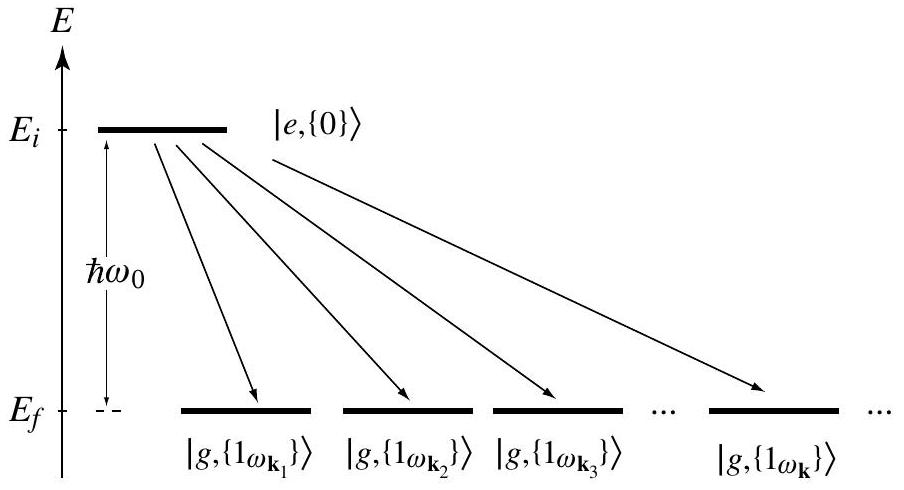
\includegraphics[alt={},max width=\textwidth]{0781daed-441b-41f1-a5d4-fc13c7f71e63-2_490_904_164_202}
\captionsetup{labelformat=empty}
\caption{Figure 8.5 Transition from an initial state $|i\rangle=|e,\{0\}\rangle$ to a set of final states $|f\rangle=\left|g,\left\{1_{\omega_{\mathbf{k}}}\right\}\right\rangle$. All the final states have the same energy. The difference between initial and final energies is $\left(E_{i}-E_{f}\right)=\hbar \omega_{0}$. The states are products of atomic states $(|e\rangle$ or $|g\rangle)$ and single-photon states $\left(|\{0\}\rangle\right.$ or $\left.\left|\left\{1_{\omega_{\mathbf{k}}}\right\}\right\rangle\right)$. The number of distinct final single-photon states is defined by the partial local density of states $\rho_{\mu}\left(\mathbf{r}_{0}, \omega_{0}\right)$, with $\mathbf{r}_{0}$ being the origin of the two-level system.}
\end{center}
\end{figure}

According to Fermi's Golden Rule $\gamma$ is given by


\begin{equation*}
\left.\gamma=\frac{2 \pi}{\hbar^{2}} \sum_{f}\left|\langle f| \hat{H}_{\mathrm{I}}\right| i\right\rangle\left.\right|^{2} \delta\left(\omega_{i}-\omega_{f}\right), \tag{8.89}
\end{equation*}


where $\hat{H}_{\mathrm{I}}=-\hat{\boldsymbol{\mu}} \cdot \hat{\mathbf{E}}$ is the interaction Hamiltonian in the dipole approximation. Notice that all $\omega_{f}$ are identical. Using the expression for $\hat{H}_{\mathrm{I}}$ we can substitute as follows:


\begin{equation*}
\left.\left|\langle f| \hat{H}_{\mathrm{I}}\right| i\right\rangle\left.\right|^{2}=\langle f| \hat{\boldsymbol{\mu}} \cdot \hat{\mathbf{E}}|i\rangle^{*}\langle f| \hat{\boldsymbol{\mu}} \cdot \hat{\mathbf{E}}|i\rangle=\langle i| \hat{\boldsymbol{\mu}} \cdot \hat{\mathbf{E}}|f\rangle\langle f| \hat{\boldsymbol{\mu}} \cdot \hat{\mathbf{E}}|i\rangle \tag{8.90}
\end{equation*}


Let us represent the electric field operator $\hat{\mathbf{E}}$ at $\mathbf{r}=\mathbf{r}_{0}$ as [2]


\begin{equation*}
\hat{\mathbf{E}}=\sum_{\mathbf{k}}\left[\mathbf{E}_{\mathbf{k}}^{+} \hat{a}_{\mathbf{k}}(t)+\mathbf{E}_{\mathbf{k}}^{-} \hat{a}_{\mathbf{k}}^{\dagger}(t)\right], \tag{8.91}
\end{equation*}


where


\begin{equation*}
\hat{a}_{\mathbf{k}}^{\dagger}(t)=\hat{a}_{\mathbf{k}}^{\dagger}(0) \exp \left(\mathrm{i} \omega_{\mathbf{k}} t\right), \quad \hat{a}_{\mathbf{k}}(t)=\hat{a}_{\mathbf{k}}(0) \exp \left(-\mathrm{i} \omega_{\mathbf{k}} t\right) \tag{8.92}
\end{equation*}


Here, $\hat{a}_{\mathbf{k}}(0)$ and $\hat{a}_{\mathbf{k}}^{\dagger}(0)$ are the annihilation and creation operators, respectively. The sum over $\mathbf{k}$ refers to summation over all modes. $\omega_{\mathbf{k}}$ denotes the frequency of mode k. The spatially dependent complex fields $\mathbf{E}_{\mathbf{k}}^{+}=\left(\mathbf{E}_{\mathbf{k}}^{-}\right)^{*}$ are the positive and negative frequency parts of the complex field $\mathbf{E}_{\mathbf{k}}$. For a two-level atomic system with\\
the ground state $|g\rangle$ and the excited state $|e\rangle$, the dipole moment operator $\hat{\boldsymbol{\mu}}$ can be written as


\begin{equation*}
\hat{\boldsymbol{\mu}}=\boldsymbol{\mu}\left[\hat{r}^{+}+\hat{r}\right], \text { with } \hat{r}^{+}=|e\rangle\langle g| \text { and } \hat{r}=|g\rangle\langle e| . \tag{8.93}
\end{equation*}


In this notation, $\boldsymbol{\mu}$ is simply the transition dipole moment, which is assumed to be real, i.e. $\langle g| \hat{\boldsymbol{\mu}}|e\rangle=\langle e| \hat{\boldsymbol{\mu}}|g\rangle$. Using the expressions for $\hat{\mathbf{E}}$ and $\hat{\boldsymbol{\mu}}$, the interaction Hamiltonian takes on the form


\begin{equation*}
-\hat{\boldsymbol{\mu}} \cdot \hat{\mathbf{E}}=-\sum_{\mathbf{k}} \boldsymbol{\mu} \cdot\left[\mathbf{E}_{\mathbf{k}}^{+} \hat{r}^{+} \hat{a}_{\mathbf{k}}(t)+\mathbf{E}_{\mathbf{k}}^{-} \hat{r} \hat{a}_{\mathbf{k}}^{\dagger}(t)+\mathbf{E}_{\mathbf{k}}^{+} \hat{r} \hat{a}_{\mathbf{k}}(t)+\mathbf{E}_{\mathbf{k}}^{-} \hat{r}^{+} \hat{a}_{\mathbf{k}}^{\dagger}(t)\right] . \tag{8.94}
\end{equation*}


We now define the initial and final state of the combined system "field + atom" as


\begin{align*}
|i\rangle & =|e,\{0\}\rangle \quad=|e\rangle|\{0\}\rangle  \tag{8.95}\\
|f\rangle & =\left|g,\left\{1_{\omega_{\mathbf{k}^{\prime}}}\right\}\right\rangle=|g\rangle\left|\left\{1_{\omega_{\mathbf{k}^{\prime}}}\right\}\right\rangle, \tag{8.96}
\end{align*}


respectively. Here, $|\{0\}\rangle$ denotes the zero-photon state, and $\left|\left\{1_{\omega_{\mathbf{k}^{\prime}}}\right\}\right\rangle$ designates the one-photon state associated with mode $\mathbf{k}^{\prime}$ and frequency $\omega_{0}=\left(E_{\mathrm{e}}-E_{\mathrm{g}}\right) / \hbar, E_{\mathrm{e}}$ and $E_{\mathrm{g}}$ being the energies of excited state and ground state, respectively. Thus, the final states in Eq. (8.89) are associated with the different modes $\mathbf{k}^{\prime}$. Operating with $\hat{\boldsymbol{\mu}} \cdot \hat{\mathbf{E}}$ on state $|i\rangle$ leads to


\begin{equation*}
\hat{\boldsymbol{\mu}} \cdot \hat{\mathbf{E}}|i\rangle=\boldsymbol{\mu} \cdot \sum_{\mathbf{k}} \mathbf{E}_{\mathbf{k}}^{-} \mathrm{e}^{\mathrm{i} \omega_{\mathbf{k}} t}\left|g,\left\{1_{\omega_{\mathbf{k}}}\right\}\right\rangle, \tag{8.97}
\end{equation*}


where we used $\hat{a}_{\mathbf{k}}^{\dagger}(0)|\{0\}\rangle=\left|\left\{1_{\omega_{\mathbf{k}}}\right\}\right\rangle$. Operating with $\langle f|$ gives


\begin{equation*}
\langle f| \hat{\boldsymbol{\mu}} \cdot \hat{\mathbf{E}}|i\rangle=\boldsymbol{\mu} \cdot \sum_{\mathbf{k}} \mathbf{E}_{\mathbf{k}}^{-} \mathrm{e}^{\mathrm{i} \omega_{\mathbf{k}} t}\left\langle g,\left\{1_{\omega_{\mathbf{k}^{\prime}}}\right\} \mid g,\left\{1_{\omega_{\mathbf{k}}}\right\}\right\rangle, \tag{8.98}
\end{equation*}


where we used $\hat{a}_{\mathbf{k}}(0)\left|\left\{1_{\omega_{\mathbf{k}}}\right\}\right\rangle=\{0\}$. A similar procedure leads to


\begin{equation*}
\langle i| \hat{\boldsymbol{\mu}} \cdot \hat{\mathbf{E}}|f\rangle=\boldsymbol{\mu} \cdot \sum_{\mathbf{k}} \mathbf{E}_{\mathbf{k}}^{+} \mathrm{e}^{-\mathrm{i} \omega_{\mathbf{k}} t}\left\langle g,\left\{1_{\omega_{\mathbf{k}}}\right\} \mid g,\left\{1_{\omega_{\mathbf{k}^{\prime}}}\right\}\right\rangle \tag{8.99}
\end{equation*}


The matrix elements can now be introduced into Eqs. (8.90) and (8.89). Expressing the sum over the final states as a sum over the modes $\mathbf{k}^{\prime}$ the transition rate becomes


\begin{align*}
\gamma= & \frac{2 \pi}{\hbar^{2}} \sum_{\mathbf{k}} \sum_{\mathbf{k}^{\prime \prime}}\left[\boldsymbol{\mu} \cdot \mathbf{E}_{\mathbf{k}^{\prime \prime}}^{+} \mathbf{E}_{\mathbf{k}}^{-} \cdot \boldsymbol{\mu}\right] \mathrm{e}^{\mathrm{i}\left(\omega_{\mathbf{k}}-\omega_{\mathbf{k}^{\prime \prime}}\right) t}  \tag{8.100}\\
& \times \sum_{\mathbf{k}^{\prime}}\left\langle g,\left\{1_{\omega_{\mathbf{k}^{\prime \prime}}}\right\} \mid g,\left\{1_{\omega_{\mathbf{k}^{\prime}}}\right\}\right\rangle\left\langle g,\left\{1_{\omega_{\mathbf{k}^{\prime}}}\right\} \mid g,\left\{1_{\omega_{\mathbf{k}}}\right\}\right\rangle \delta\left(\omega_{\mathbf{k}^{\prime}}-\omega_{0}\right) .
\end{align*}


Because of orthogonality, the only non-vanishing terms are those for which $\mathbf{k}^{\prime}= \mathbf{k}^{\prime \prime}=\mathbf{k}$, which leads to the simple expression


\begin{equation*}
\gamma=\frac{2 \pi}{\hbar^{2}} \sum_{\mathbf{k}}\left[\boldsymbol{\mu} \cdot\left(\mathbf{E}_{\mathbf{k}}^{+} \mathbf{E}_{\mathbf{k}}^{-}\right) \cdot \boldsymbol{\mu}\right] \delta\left(\omega_{\mathbf{k}}-\omega_{0}\right) . \tag{8.101}
\end{equation*}


Here, $\mathbf{E}_{\mathbf{k}}^{+} \mathbf{E}_{\mathbf{k}}^{-}$denotes the outer product, i.e. the result is a $3 \times 3$ matrix. For later purposes it is convenient to rewrite this expression in terms of normal modes $\mathbf{u}_{\mathbf{k}}$ defined as


\begin{equation*}
\mathbf{E}_{\mathbf{k}}^{+}=\sqrt{\frac{\hbar \omega_{\mathbf{k}}}{2 \varepsilon_{0}}} \mathbf{u}_{\mathbf{k}}, \quad \mathbf{E}_{\mathbf{k}}^{-}=\sqrt{\frac{\hbar \omega_{\mathbf{k}}}{2 \varepsilon_{0}}} \mathbf{u}_{\mathbf{k}}^{*} \tag{8.102}
\end{equation*}


Because the delta function imposes $\omega_{\mathbf{k}}=\omega_{0}$ the decay rate can be written as


\begin{equation*}
\gamma=\frac{2 \omega}{3 \hbar \varepsilon_{0}}|\boldsymbol{\mu}|^{2} \rho_{\mu}\left(\mathbf{r}_{0}, \omega_{0}\right), \quad \rho_{\mu}\left(\mathbf{r}_{0}, \omega_{0}\right)=3 \sum_{\mathbf{k}}\left[\mathbf{n}_{\mu} \cdot\left(\mathbf{u}_{\mathbf{k}} \mathbf{u}_{\mathbf{k}}^{*}\right) \cdot \mathbf{n}_{\mu}\right] \delta\left(\omega_{\mathbf{k}}-\omega_{0}\right), \tag{8.103}
\end{equation*}


where we introduced the partial local density of states $\rho_{\mu}\left(\mathbf{r}_{0}, \omega_{0}\right)$, which will be discussed in the next section. The dipole moment has been decomposed as $\boldsymbol{\mu}=\mu \mathbf{n}_{\mu}$ with $\mathbf{n}_{\mu}$ being the unit vector in the direction of $\boldsymbol{\mu}$. The above equation for $\gamma$ is our main result. The delta-function in the expression suggests that we need to integrate over a finite distribution of final frequencies. However, even for a single final frequency, the apparent singularity introduced through $\delta\left(\omega_{\mathbf{k}}-\omega_{0}\right)$ is compensated by the normal modes whose magnitude tends to zero for a sufficiently large mode volume. In any case, it is convenient to get rid of these singularities by representing $\rho_{\mu}\left(\mathbf{r}_{0}, \omega_{0}\right)$ in terms of the Green's function instead of normal modes.

\subsection*{8.4.2 Spontaneous decay and Green's dyadics}
We aim to derive an important relationship between the normal modes $\mathbf{u}_{\mathbf{k}}$ and the dyadic Green's function $\overleftrightarrow{\mathbf{G}}$. Subsequently, this relationship is used to express the spontaneous decay rate $\gamma$ and to establish an elegant expression for the local density of states. While we suppressed the explicit position dependence of $\mathbf{u}_{\mathbf{k}}$ in the previous section for notational convenience, it is essential in the current context to carry all the arguments. The normal modes defined in the previous section satisfy the wave equation


\begin{equation*}
\nabla \times \nabla \times \mathbf{u}_{\mathbf{k}}\left(\mathbf{r}, \omega_{\mathbf{k}}\right)-\frac{\omega_{\mathbf{k}}^{2}}{c^{2}} \mathbf{u}_{\mathbf{k}}\left(\mathbf{r}, \omega_{\mathbf{k}}\right)=0 \tag{8.104}
\end{equation*}


and they fulfill the orthogonality relation


\begin{equation*}
\int \mathbf{u}_{\mathbf{k}}\left(\mathbf{r}, \omega_{\mathbf{k}}\right) \cdot \mathbf{u}_{\mathbf{k}^{\prime}}^{*}\left(\mathbf{r}, \omega_{\mathbf{k}^{\prime}}\right) \mathrm{d}^{3} \mathbf{r}=\delta_{\mathbf{k k}^{\prime}} \tag{8.105}
\end{equation*}


where the integration runs over the entire mode volume. $\delta_{\mathbf{k k}^{\prime}}$ is the Kronecker delta and $\overleftrightarrow{\mathbf{I}}$ the unit dyad. We now expand the Green's function $\overleftrightarrow{\mathbf{G}}$ in terms of the normal modes as


\begin{equation*}
\overleftrightarrow{\mathbf{G}}\left(\mathbf{r}, \mathbf{r}^{\prime} ; \omega\right)=\sum_{\mathbf{k}} \mathbf{A}_{\mathbf{k}}\left(\mathbf{r}^{\prime}, \omega\right) \mathbf{u}_{\mathbf{k}}\left(\mathbf{r}, \omega_{\mathbf{k}}\right) \tag{8.106}
\end{equation*}


where the vectorial expansion coefficients $\mathbf{A}_{\mathbf{k}}$ have yet to be determined.\\
We recall the definition of the Green's function (cf. Eq. (2.78))


\begin{equation*}
\nabla \times \nabla \times \overleftrightarrow{\mathbf{G}}\left(\mathbf{r}, \mathbf{r}^{\prime} ; \omega\right)-\frac{\omega^{2}}{c^{2}} \overleftrightarrow{\mathbf{G}}\left(\mathbf{r}, \mathbf{r}^{\prime} ; \omega\right)=\overleftrightarrow{\mathbf{I}} \delta\left(\mathbf{r}-\mathbf{r}^{\prime}\right) \tag{8.107}
\end{equation*}


To determine the coefficients $\mathbf{A}_{\mathbf{k}}$ we substitute the expansion for $\overleftrightarrow{\mathbf{G}}$ and obtain


\begin{equation*}
\sum_{\mathbf{k}} \mathbf{A}_{\mathbf{k}}\left(\mathbf{r}^{\prime}, \omega\right)\left[\nabla \times \nabla \times \mathbf{u}_{\mathbf{k}}\left(\mathbf{r}, \omega_{\mathbf{k}}\right)-\frac{\omega^{2}}{c^{2}} \mathbf{u}_{\mathbf{k}}\left(\mathbf{r}, \omega_{\mathbf{k}}\right)\right]=\overleftrightarrow{\mathbf{I}} \delta\left(\mathbf{r}-\mathbf{r}^{\prime}\right) \tag{8.108}
\end{equation*}


Using Eq. (8.104) we can rewrite the latter as


\begin{equation*}
\sum_{\mathbf{k}} \mathbf{A}_{\mathbf{k}}\left(\mathbf{r}^{\prime}, \omega\right)\left[\frac{\omega_{\mathbf{k}}^{2}}{c^{2}}-\frac{\omega^{2}}{c^{2}}\right] \mathbf{u}_{\mathbf{k}}\left(\mathbf{r}, \omega_{\mathbf{k}}\right)=\overleftrightarrow{\mathbf{I}} \delta\left(\mathbf{r}-\mathbf{r}^{\prime}\right) \tag{8.109}
\end{equation*}


Multiplying on both sides with $\mathbf{u}_{\mathbf{k}^{\prime}}^{*}$, integrating over the mode volume and making use of the orthogonality relation leads to


\begin{equation*}
\mathbf{A}_{\mathbf{k}^{\prime}}\left(\mathbf{r}^{\prime}, \omega\right)\left[\frac{\omega_{\mathbf{k}^{\prime}}^{2}}{c^{2}}-\frac{\omega^{2}}{c^{2}}\right]=\mathbf{u}_{\mathbf{k}^{\prime}}^{*}\left(\mathbf{r}^{\prime}, \omega_{\mathbf{k}}\right) \tag{8.110}
\end{equation*}


Substituting this expression back into Eq. (8.106) leads to the desired expansion for $\overleftrightarrow{\mathbf{G}}$ in terms of the normal modes


\begin{equation*}
\overleftrightarrow{\mathbf{G}}\left(\mathbf{r}, \mathbf{r}^{\prime} ; \omega\right)=\sum_{\mathbf{k}} c^{2} \frac{\mathbf{u}_{\mathbf{k}}^{*}\left(\mathbf{r}^{\prime}, \omega_{\mathbf{k}}\right) \mathbf{u}_{\mathbf{k}}\left(\mathbf{r}, \omega_{\mathbf{k}}\right)}{\omega_{\mathbf{k}}^{2}-\omega^{2}} \tag{8.111}
\end{equation*}


To proceed we make use of the following mathematical identity which can be easily proved by complex contour integration


\begin{equation*}
\lim _{\eta \rightarrow 0} \operatorname{Im}\left\{\frac{1}{\omega_{\mathbf{k}}^{2}-(\omega+\mathrm{i} \eta)^{2}}\right\}=\frac{\pi}{2 \omega_{\mathbf{k}}}\left[\delta\left(\omega-\omega_{\mathbf{k}}\right)-\delta\left(\omega+\omega_{\mathbf{k}}\right)\right] \tag{8.112}
\end{equation*}


Multiplying on both sides with $\mathbf{u}_{\mathbf{k}}^{*}\left(\mathbf{r}, \omega_{\mathbf{k}}\right) \mathbf{u}_{\mathbf{k}}\left(\mathbf{r}, \omega_{\mathbf{k}}\right)$ and summing over all $\mathbf{k}$ yields


\begin{equation*}
\operatorname{Im}\left\{\lim _{\eta \rightarrow 0} \sum_{\mathbf{k}} \frac{\mathbf{u}_{\mathbf{k}}^{*}\left(\mathbf{r}, \omega_{\mathbf{k}}\right) \mathbf{u}_{\mathbf{k}}\left(\mathbf{r}, \omega_{\mathbf{k}}\right)}{\omega_{\mathbf{k}}^{2}-(\omega+\mathrm{i} \eta)^{2}}\right\}=\frac{\pi}{2} \sum_{\mathbf{k}} \frac{1}{\omega_{\mathbf{k}}} \mathbf{u}_{\mathbf{k}}^{*}\left(\mathbf{r}, \omega_{\mathbf{k}}\right) \mathbf{u}_{\mathbf{k}}\left(\mathbf{r}, \omega_{\mathbf{k}}\right) \delta\left(\omega-\omega_{\mathbf{k}}\right), \tag{8.113}
\end{equation*}


where we dropped the term $\delta\left(\omega+\omega_{\mathbf{k}}\right)$ because we are concerned only with positive frequencies. By comparison with Eq. (8.111), the expression in brackets on the left hand side can be identified with the Green's function evaluated at its origin $\mathbf{r}=\mathbf{r}^{\prime}$.

Furthermore, the delta function on the right hand side restricts all values of $\omega_{\mathbf{k}}$ to $\omega$, which allows us to move the first factor out of the sum. We therefore obtain the important relationship


\begin{equation*}
\operatorname{Im}\{\overleftrightarrow{\mathbf{G}}(\mathbf{r}, \mathbf{r} ; \omega)\}=\frac{\pi c^{2}}{2 \omega} \sum_{\mathbf{k}} \mathbf{u}_{\mathbf{k}}^{*}\left(\mathbf{r}, \omega_{\mathbf{k}}\right) \mathbf{u}_{\mathbf{k}}\left(\mathbf{r}, \omega_{\mathbf{k}}\right) \delta\left(\omega-\omega_{\mathbf{k}}\right) . \tag{8.114}
\end{equation*}


We now set $\mathbf{r}=\mathbf{r}_{0}$ and $\omega=\omega_{0}$ and rewrite the decay rate $\gamma$ and the partial local density of states $\rho_{\mu}$ in Eq. (8.103) as

$$
\gamma=\frac{2 \omega_{0}}{3 \hbar \varepsilon_{0}}|\boldsymbol{\mu}|^{2} \rho_{\mu}\left(\mathbf{r}_{0}, \omega_{0}\right), \quad \rho_{\mu}\left(\mathbf{r}_{0}, \omega_{0}\right)=\frac{6 \omega_{0}}{\pi c^{2}}\left[\mathbf{n}_{\mu} \cdot \operatorname{Im}\left\{\stackrel{\leftrightarrow}{\mathbf{G}}\left(\mathbf{r}_{0}, \mathbf{r}_{0} ; \omega_{0}\right)\right\} \cdot \mathbf{n}_{\mu}\right] .
$$

This formula is the main result of this section. It allows us to calculate the spontaneous decay rate of a two-level quantum system in an arbitrary reference system. All that is needed is knowledge of the Green's dyadic for the reference system. The Green's dyadic is evaluated at its origin, which corresponds to the location of the atomic system. From a classical viewpoint this is equivalent to the electric field previously emitted by the quantum system and now arriving back at its origin. The mathematical analogy of the quantum and the classical treatments now becomes obvious when comparing Eq. (8.115) and Eq. (8.75). The latter is the classical equation for energy dissipation based on Poynting's theorem.

\begin{figure}[h]
\begin{center}
  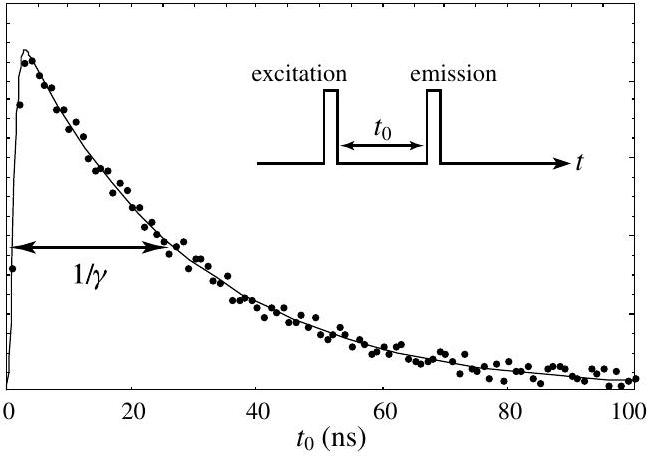
\includegraphics[alt={},max width=\textwidth]{0781daed-441b-41f1-a5d4-fc13c7f71e63-6_456_651_1191_329}
\captionsetup{labelformat=empty}
\caption{Figure 8.6 Radiative decay rate $\gamma$ of the $2 \mathrm{P}_{1 / 2}$ state of Li . The time interval $t_{0}$ between an excitation pulse and the subsequent photon count is measured and plotted in a histogram. The 1/e width of the exponential distribution corresponds to the lifetime $\tau=1 / \gamma=27.1 \mathrm{~ns}$. For $t_{0} \rightarrow 0$ the distribution falls to zero because of the finite response time of the photon detector.}
\end{center}
\end{figure}

We have expressed $\gamma$ in terms of the partial local density of states $\rho_{\mu}$, which corresponds to the number of modes per unit volume and frequency, at the origin $\mathbf{r}$ of the (point-like) quantum system, into which a photon with energy $\hbar \omega_{0}$ can be released during the spontaneous decay process. In the next section we discuss some important aspects of $\rho_{\mu}$.

\subsection*{8.4.3 Local density of states}
In situations where the transitions of the quantum system have no fixed dipole axis $\mathbf{n}_{\mu}$ and the medium is isotropic and homogeneous, the decay rate is averaged over the various orientations leading to (see Problem 8.6)


\begin{equation*}
\left\langle\mathbf{n}_{\mu} \cdot \operatorname{Im}\left\{\overleftrightarrow{\mathbf{G}}\left(\mathbf{r}_{0}, \mathbf{r}_{0} ; \omega_{0}\right)\right\} \cdot \mathbf{n}_{\mu}\right\rangle=\frac{1}{3} \operatorname{Im}\left\{\operatorname{Tr}\left[\overleftrightarrow{\mathbf{G}}\left(\mathbf{r}_{0}, \mathbf{r}_{0} ; \omega_{0}\right)\right]\right\} . \tag{8.116}
\end{equation*}


Substituting into Eq. (8.115), we find that in this case the partial local density of states $\rho_{\mu}$ becomes identical with the total local density of states $\rho$ defined as


\begin{equation*}
\rho\left(\mathbf{r}_{0}, \omega_{0}\right)=\frac{2 \omega_{0}}{\pi c^{2}} \operatorname{Im}\left\{\operatorname{Tr}\left[\overleftrightarrow{\mathbf{G}}\left(\mathbf{r}_{0}, \mathbf{r}_{0} ; \omega_{0}\right)\right]\right\}=\sum_{\mathbf{k}}\left|\mathbf{u}_{\mathbf{k}}\right|^{2} \delta\left(\omega_{\mathbf{k}}-\omega_{0}\right) \tag{8.117}
\end{equation*}


where $\operatorname{Tr}[\ldots]$ denotes the trace of the tensor in brackets. $\rho$ corresponds to the total number of electromagnetic modes per unit volume and unit frequency at a given location $\mathbf{r}_{0}$. In practice, $\rho$ has little significance because any detector or measurement relies on the translation of charge carriers from one point to another. Defining the axis between these points as $\mathbf{n}_{\mu}$ it is obvious that $\rho_{\mu}$ is of much greater practical significance as it also enters the well-known formula for spontaneous decay.

As shown earlier in Section 8.3.3, the imaginary part of $\overleftrightarrow{\mathbf{G}}$ evaluated at its origin is not singular. For example, in free space ( $\overleftrightarrow{\mathbf{G}}=\overleftrightarrow{\mathbf{G}}_{0}$ ) we have (see Problem 8.7)


\begin{equation*}
\left[\mathbf{n}_{\mu} \cdot \operatorname{Im}\left\{\overleftrightarrow{\mathbf{G}}_{0}\left(\mathbf{r}_{0}, \mathbf{r}_{0} ; \omega_{0}\right)\right\} \cdot \mathbf{n}_{\mu}\right]=\frac{1}{3} \operatorname{Im}\left\{\operatorname{Tr}\left[\overleftrightarrow{\mathbf{G}}_{0}\left(\mathbf{r}_{0}, \mathbf{r}_{0} ; \omega_{0}\right)\right]\right\}=\frac{\omega_{0}}{6 \pi c}, \tag{8.118}
\end{equation*}


where no orientational averaging has been performed. It is the symmetric form of $\overleftrightarrow{\mathbf{G}}_{0}$ that leads to this simple expression. Thus, $\rho$ and $\rho_{\mu}$ take on the well-known value of


\begin{equation*}
\rho_{0}=\frac{\omega_{0}^{2}}{\pi^{2} c^{3}} \tag{8.119}
\end{equation*}


which is the density of electromagnetic modes as encountered in blackbody radiation. The free-space spontaneous decay rate turns out to be


\begin{equation*}
\gamma_{0}=\frac{\omega_{0}^{3}|\boldsymbol{\mu}|^{2}}{3 \pi \varepsilon_{0} \hbar c^{3}}, \tag{8.120}
\end{equation*}


where $\boldsymbol{\mu}=\langle g| \hat{\boldsymbol{\mu}}|e\rangle$ denotes the transition dipole matrix element.

To summarize, the spontaneous decay rate is proportional to the partial local density of states, which depends on the transition dipole defined by the two atomic states involved in the transition. Only in homogeneous environments or after orientational averaging can $\rho_{\mu}$ be replaced by the total local density of states. This explains why a change in the environmental conditions can change the spontaneous decay rate.

\subsection*{8.5 Classical lifetimes and decay rates}
We now derive the classical picture of spontaneous decay by considering an undriven harmonically oscillating dipole. As the dipole oscillates it radiates energy according to Eq. (8.70). As a consequence, the dipole dissipates its energy into radiation and its dipole moment decreases. We are interested in calculating the time $\tau$ after which the dipole's energy decreases to $1 / \mathrm{e}$ of its initial value.

\subsection*{8.5.1 Homogeneous environment}
The equation of motion for an undriven harmonically oscillating dipole is (cf. Eq. (8.87))


\begin{equation*}
\frac{\mathrm{d}^{2}}{\mathrm{~d} t^{2}} \boldsymbol{\mu}(t)+\gamma_{0} \frac{\mathrm{~d}}{\mathrm{~d} t} \boldsymbol{\mu}(t)+\omega_{0}^{2} \boldsymbol{\mu}(t)=0 . \tag{8.121}
\end{equation*}


The natural frequency of the oscillator is $\omega_{0}$ and its damping constant is $\gamma_{0}$. The solution for $\boldsymbol{\mu}$ is


\begin{equation*}
\boldsymbol{\mu}(t)=\operatorname{Re}\left\{\boldsymbol{\mu}_{0} \mathrm{e}^{-\mathrm{i} \omega_{0} \sqrt{1-\left(\gamma_{0}^{2} / 4 \omega_{0}^{2}\right)} t} \mathrm{e}^{\gamma_{0} t / 2}\right\} . \tag{8.122}
\end{equation*}


Because of losses introduced through $\gamma_{0}$ the dipole forms a non-conservative system. The damping rate not only attenuates the dipole strength but also produces a shift in resonance frequency. In order to be able to define an average dipole energy $\bar{W}$ at any instant of time we have to make sure that the oscillation amplitude stays constant over one period of oscillation. In other words, we require


\begin{equation*}
\gamma_{0} \ll \omega_{0} . \tag{8.123}
\end{equation*}


The average energy of a harmonic oscillator is the sum of the average kinetic and potential energy. At time $t$ this average energy reads as ${ }^{8}$


\begin{equation*}
\bar{W}(t)=\frac{m}{2 q^{2}}\left[\omega_{0}^{2} \mu^{2}(t)+\dot{\mu}^{2}(t)\right]=\frac{m \omega_{0}^{2}}{2 q^{2}}\left|\boldsymbol{\mu}_{0}\right|^{2} \mathrm{e}^{-\gamma_{0} t}, \tag{8.124}
\end{equation*}


\footnotetext{${ }^{8}$ This is easily derived by setting $\mu=q x, \omega_{0}^{2}=c / m$ and using the expressions $m \dot{x}^{2} / 2$ and $c x^{2} / 2$ for the kinetic and potential energy, respectively.
}
\end{document}